\cleardoublepage
\chapter{基于区块链存储系统的测量与研究}
\label{sec:baseline}
本章将深入探讨基于区块链的物联网时序数据存储系统的基础架构,并对该系统进行了全面的测量研究。
基于测量研究,本文发现聚合存储能够显著降低存储延迟,但在物联网场景中较为常见的范围查询中,同时也引入了查询延迟的问题。
本章进一步分析了导致查询性能不佳的根本原因,包括查询跨越多个聚合单元、存储节点选择不当以及庞大的数据完整性证明。
为了解决这些问题,本文提出了TimeChain架构,这是一种新颖的、基于区块链的物联网时间序列数据存储系统。
本章介绍了TimeChain系统的核心模块,包括数据批处理模块、存储节点选择模块和数据验证模块。
这些模块共同作用,旨在减少查询延迟、提高数据存储的效率和安全性。

\section{基于区块链存储系统的架构}

\begin{figure}[t]
    \centering
    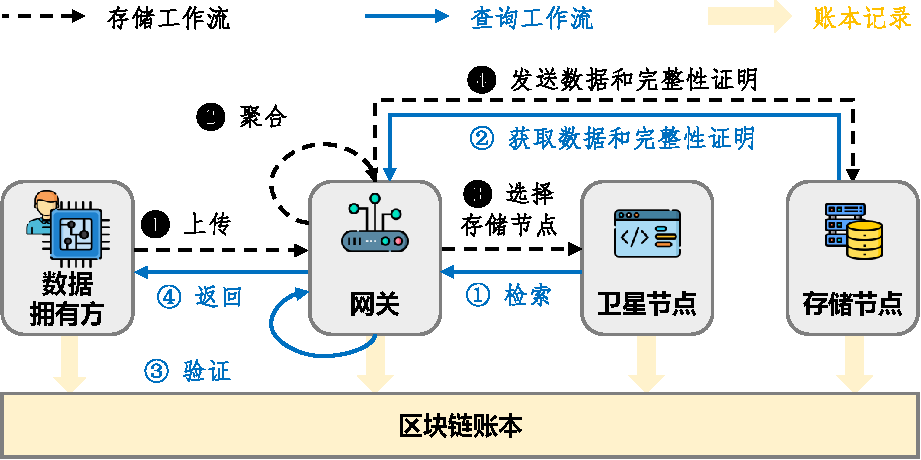
\includegraphics[width=0.9\linewidth]{figures/timechain/measurement_workflow.pdf}
    \caption{基于区块链的存储系统的工作流}
    \label{fig:workflow}
\end{figure}

为了提高基于区块链的分布式数据库的性能,本文提出了一种基本的链下存储系统,并对其进行了测量研究。
如\autoref{fig:workflow}所示,一个基于区块链的基本分布式存储系统有四个主要角色,即\textbf{数据拥有者}、\textbf{网关}、\textbf{卫星}和\textbf{存储提供商}。

\begin{itemize}
    \item[$\bullet$] \textbf{数据拥有者}:数据拥有者是数据的生成者和消费者,他们发起上传和查询数据的请求。
    \item[$\bullet$] \textbf{网关}:网关是数据拥有者与存储提供商之间的中间层,负责数据的上传和下载。
    \item[$\bullet$] \textbf{卫星}:与Storj~\cite{storj2018storj}和FileCoin~\cite{bauer2022filecoin}类似,卫星是一个智能合约,负责协调数据拥有者和存储提供商之间的交互。
    它们提供文件审计(检查)或可检索性(Proofs of Retrievability,POR)相关功能和对存储支付等操作的处理。
    \item[$\bullet$] \textbf{存储提供商}:存储提供商是存储数据的节点,通过提供存储服务获得奖励。
    为了使存储提供商能够通过灵活的查询快速向数据拥有者提供完整性证明,数据完整性证明也需要存储在存储提供商中,便于通过默克尔树的路径直接快速组装成完整性证明。
    存储提供商的服务信息,如剩余存储空间,将与交互记录一起记录在分布式账本中,以确保安全。
\end{itemize}

一般来说,数据存储和查询过程可以概括如下:

\textbf{数据存储:}
\ding{182}\textit{上传}:
数据拥有者通过网关接口上传数据。
\ding{183}\textit{聚合}:
网关接收到数据后,会对时间序列数据进行批处理。
这一步骤涉及到将多个数据点聚合在一起,并为每批数据生成数据完整性证明,这对于确保数据在存储和后续查询过程中的完整性至关重要。
\ding{184}\textit{选择存储节点}:
在聚合数据后,卫星节点介入,帮助网关识别和选择最佳的存储节点。
这一步骤基于一系列选择策略,考虑如节点的信誉、存储空间和地理位置等因素,以确保数据被存储在最可靠和最经济的节点上。
\ding{185}\textit{发送数据和完整性证明}:
一旦确定了最佳存储节点,原始传感器数据及其完整性证明将被发送到这些节点。
同时,数据批的元数据被记录在分布式账本中,利用区块链的不可篡改性确保数据的透明性和可追溯性。

\textbf{数据查询:}
\ding{172}\textit{检索}:
当数据拥有者需要访问他们的数据时,他们通过网关发起数据下载请求。
网关随后与卫星节点交互,以检索存储提供商的位置信息。
\ding{173}\textit{获取数据和完整性证明}:
网关根据从卫星节点获得的位置信息,从存储提供商处获取所需的数据及其完整性证明。
这一步骤确保了数据在传输过程中的安全性和完整性。
\ding{174}\textit{验证}:
在获取数据后,网关将通过检查数据完整性证明来验证下载数据的完整性,确保数据未被篡改且准确无误。
\ding{175}\textit{返回}:
最后,经过验证的数据将通过网关安全地返回给数据拥有者,完成整个数据查询流程。

\section{基于区块链存储系统的测量}
在本节中,本文进行了一项初步测量,以评估基于区块链的基本存储系统的性能。
本文使用Hyperledger Fabric作为区块链平台,IPFS作为文件存储系统,实现了上述基本存储系统。
该测试网络由5个节点组成,其中1个节点是网关,4个节点是卫星。
为了更准确地模拟真实世界中的存储网络环境,本文基于真实世界的数据存储网络模拟了一个包括320个存储节点的网络,其中包括189个真实存储提供商~\cite{corneo2021surrounded}和131个模拟提供商(代表提供闲置存储的个人提供商)。
为了确保实验结果的准确性,网关与这些模拟提供商之间的传输延迟是通过一个基于现有研究的线性回归模型~\cite{ziviani2005improving}进行预测的。

\begin{figure*}[t]
    \centering
    \begin{minipage}{1\linewidth}
	    \centering
        \subfigure[存储时延]{
            \centering
            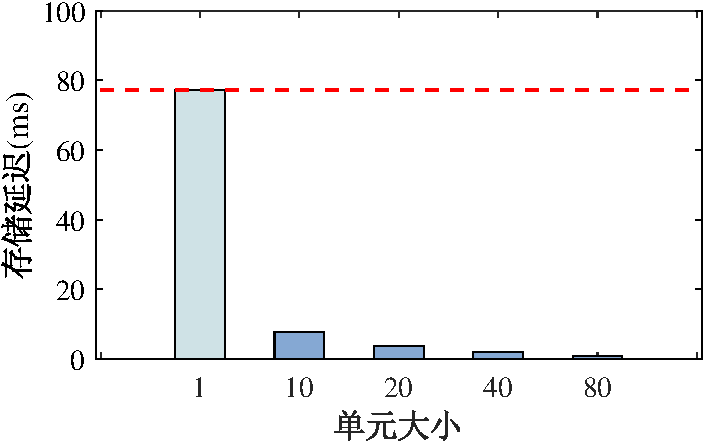
\includegraphics[width=0.48\textwidth]{figures/timechain/measurement_storage.pdf}
            \label{fig:measurement_storage}
        }
        \hfill
        \subfigure[查询时延]{
            \centering
            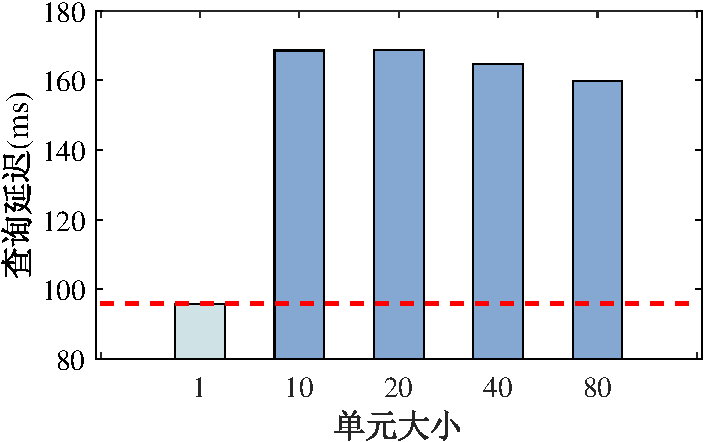
\includegraphics[width=0.48\textwidth]{figures/timechain/measurement_query.pdf}
            \label{fig:measurement_query}
        }
        \caption{区块链存储系统的性能} 
    \end{minipage}
\end{figure*}

\textbf{存储性能。}
在本文设置的系统中,数据拥有者每秒生成20个56字节的数据包,并在20秒内存储它们。
这一设置模拟了物联网场景中常见的高频数据生成和存储需求。
存储性能结果如图\autoref{fig:measurement_storage}所示。
与单独存储每个数据相比,批存储将延迟减少到约37.4分之一,且随着聚合单元增大,存储延迟逐渐降低。
这主要是因为较大的聚合单元规模减少了链上操作和数据传输的次数,从而降低了存储延迟。

\textbf{查询性能。}
然后,本文测试范围查询的性能,如图\autoref{fig:measurement_query}所示。
不幸的是,结果显示,相对于存储单个数据而言,批处理存储解决方案的查询性能相对较差。
具体而言,该方案在不同聚合单元大小下的平均查询延迟为165.4ms,这一延迟水平对于许多对实时性要求较高的物联网应用场景来说是难以接受的。
例如,在自动驾驶领域,系统需要在极短时间内做出决策,其延迟要求通常低于50ms~\cite{caesar2020nuscenes};而在地震监测场景中,为了及时发出警报并采取应对措施,系统的延迟要求通常低于100ms~\cite{bhatia2023artificial}。
由此可见,尽管批处理存储方案在降低存储开销方面具有显著优势,但在查询效率上仍存在较大的改进空间,尤其是在面对高频查询和低延迟需求的物联网应用时。

\section{性能瓶颈的根本原因}
为了找出该方案查询性能不佳的原因,本文进行了深入研究,并将原因总结为以下三点:

\begin{figure*}[t]
    \centering
    \begin{minipage}{1\linewidth}
	    \centering
        \subfigure[查询跨越多个聚合单元]{
            \centering
            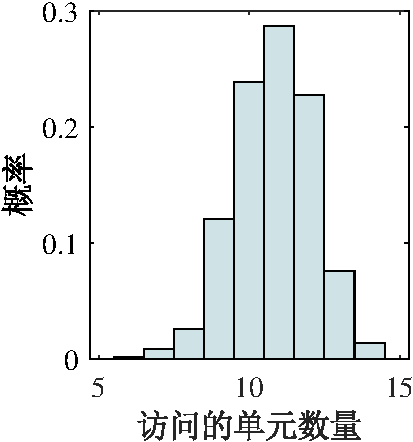
\includegraphics[width=0.3\textwidth]{figures/timechain/batch_cdf.pdf}
            \label{fig:batch_cdf}
        }
        \hfill
        \subfigure[不正确的存储节点选择]{
            \centering
            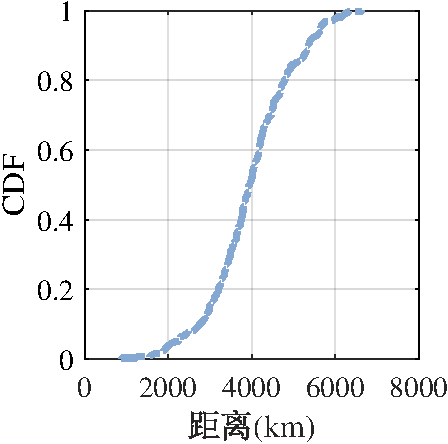
\includegraphics[width=0.32\textwidth]{figures/timechain/dis_cdf.pdf}
            \label{fig:dis_cdf}
        }
        \hfill
        \subfigure[传输数据较大]{
            \centering
            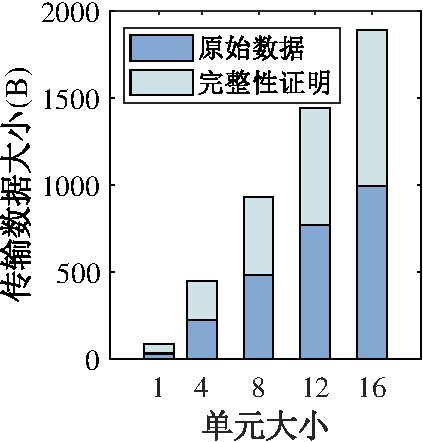
\includegraphics[width=0.3\textwidth]{figures/timechain/proof_size_cdf.pdf}
            \label{fig:proof_size_cdf}
        }
        \caption{性能低下的根本原因} 
    \end{minipage}
\end{figure*}

\begin{itemize}
    \item \textbf{范围查询跨越多个批处理单元。}
    时间序列数据的查询通常包含多个数据点,如范围查询、聚合查询、过滤查询等。
    如果批处理不当,单个查询可能会跨越多个批处理单元。
    本文使用现有的数据集YCSB~\cite{barata2014ycsb}评估每个查询所跨越的批处理单元数量。
    如图\autoref{fig:batch_cdf}所示,超过84.25\%的查询跨越了10个批处理单元。
    当这些批处理单元被存储在不同的节点上时,向不同存储节点获取数据的过程将引入额外的查询和传输延迟。

    \item \textbf{存储节点选择不当。}
    在这个测量中,本文发现传输延迟占总查询延迟的很大一部分。
    如图\autoref{fig:dis_cdf}所示,世界各地存储节点的距离存在很大差异,导致节点之间的传输延迟存在很大差异。
    选择非常远的存储节点将导致传输延迟显著增加。
    此外,在整个存储网络中存在恶意节点的情况下,尽管最终选择的节点可能传输延迟较小,然而,由于恶意节点的存在,数据的完整性可能会受到威胁,从而无法提供完整的数据存储服务。

    \item \textbf{完整性证明数据量大。}
    在数据获取阶段中,存储提供商为了证明数据的完整性,需要生成数据完整性证明并发送给数据拥有者。
    为了使存储提供商能够通过灵活的查询快速向数据拥有者提供完整性证明,数据完整性证明也需要与存储提供商一起存储。
    图\autoref{fig:proof_size_cdf}显示了在数据获取阶段时,总传输数据量的各组成部分。
    从图中可以看出,数据完整性证明大小占接收数据的48.8\%,几乎是接收数据的一半。
    当网络繁忙时,大量的完整性证明数据传输会增加网络传输延迟。
\end{itemize}

\section{高效的链下存储架构}
\label{sec:design}

\begin{figure}[t]
    \centering
    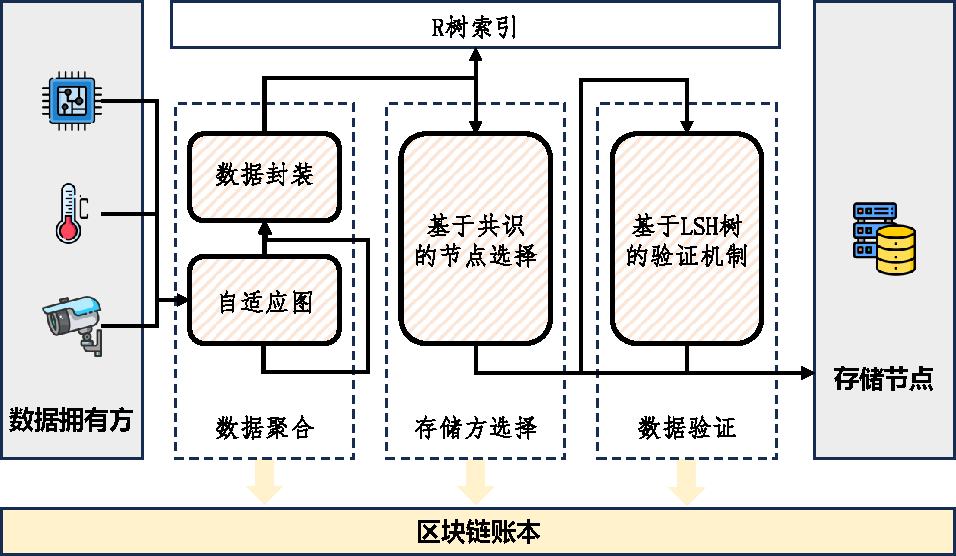
\includegraphics[width=1\linewidth]{figures/timechain/arch.pdf}
    \caption{TimeChain架构}
    \label{fig:architecture}
\end{figure}

为了提高区块链存储系统的查询性能,本文设计了一种基于区块链的新型物联网时间序列数据存储系统,TimeChain。
\autoref{fig:architecture}显示了TimeChain的架构。
TimeChain中的模块包括数据聚合、存储方选择、数据验证、R树索引和区块链账本。
TimeChain建立在区块链平台上,所有操作都记录在分布式账本上,以方便数据的审计和追踪。
TimeChain的索引结构是R树,可以加速物联网场景中常用的时空聚合搜索。

原始数据经过数据聚合模块,确定哪些数据被放在一个聚合单元中;经过存储方选择模块,确定聚合单元的存储位置。
这些信息将被放在R树中,以便快速查询。
接下来,本文介绍TimeChain的关键模块。

\textbf{数据聚合模块:}
本文的测量研究表明,不正确的聚合方法会增加查询的跨单元数量,从而增加网络传输延迟。
本文构建了一个自适应的无向加权图(Undirected Weighted Graph,UWG),以基于数据拥有者的历史查询准确捕获用户查询信息(§-\ref{sec:UWG})。
该图可以根据数据拥有者的历史查询记录动态更新,具有良好的适应性和准确性。
基于本文构建的UWG,本文将数据打包成批处理单元的问题转换为聚类问题~\cite{xu2005survey},根据用户的查询请求将所有原始数据划分为多个聚类。
解决聚类问题的传统算法有很多,如K-means~\cite{kanungo2002efficient}、GMM~\cite{he2010laplacian}等。
然而,这种传统的聚类算法不适合分割物联网设备生成的数据。
这是因为在TimeChain中,用户的查询没有遵循特定的特征,这可能会导致数据图的聚类形成复杂的形状,而不是常见的圆形。
此外,传统的聚类算法需要将所有数据划分为固定数量的集合,但并非所有集合都等于批大小,这将给索引查询带来额外的开销。
因此,本文使用谱聚类算法来打包数据(§-\ref{sec:ratiocut}),这非常适合处理不规则和非固定数量的聚类。

\textbf{存储方选择模块:}
存储节点的\textit{选择}至关重要。
正如本文之前在图\autoref{fig:dis_cdf}中发现的那样,存储节点和网关之间的距离会影响数据访问延迟。
此外,对于链下存储系统,存储空间不足的节点或恶意节点可能会导致数据丢失、篡改或服务中断,进而影响整个系统的安全性和稳定性。
因此,本文在存储节点的评估过程中综合考虑距离和历史服务记录等信息。
存储节点\textit{选择过程的安全性}也非常重要。
Storj~\cite{storj2018storj}、CoopEdge~\cite{yuan2021coopedge}和PipeEdge~\cite{yuan2023pipeedge}通过一组固定的节点选择服务节点,并通过区块链确认决策。
换句话说,他们集中决策,但仍然面临单点失败的威胁。
然而,使用类似于PBFT~\cite{li2020scalable}的投票机制,节点选择过程通常需要多轮任务计算和消息广播。
如果共识过程和节点选择过程完全解耦,系统安全将受到威胁。
为了解决这个问题,本文将节点选择过程与共识相结合,提出了一种基于共识的节点选择机制(§-\ref{sec:consensus})。
本文也进一步分析了该机制的安全性。

\textbf{数据验证模块:}
从之前的测量结果中本文可以发现,传输的数据中接近一半是数据完整性证明。
数据完整性证明被组织为默克尔树的形式,它是由一系列哈希构建的。
在默克尔树中,非叶子节点的哈希数几乎等于原始数据点的数量。
由于物联网数据单元的大小大约等于哈希值,这意味着需要发送以验证数据的数据量几乎是原始数据的两倍。
在这样的数据传输过程中,减小数据证明的大小是一个挑战。
通过分析物联网数据,本文观察到物联网数据变化缓慢,在短时间内很少出现突然变化。
对于这些相似的数据,LSH算法可以从相似的原始数据中生成相似的哈希结果。
LSH算法确保类似的物联网数据即使在哈希后也保持相似。
因此,本文提出了一种新的基于LSH树的验证机制(§-\autoref{sec:lsh}),该机制采用LSH而不是传统默克尔树中使用的通用哈希。
通过差分传输LSH哈希值,可以显著减小传输数据的大小。

\section{本章小结}
受链下存储启发,本章先提出了一种基于区块链的物联网时序数据基本存储系统。
对于这个基本系统,本章进行了一些性能测试,发现该系统确实可以降低存储延迟,但查询延迟较高。
本章进一步分析了查询性能不佳的根本原因,并针对性能瓶颈提出了高效链下存储系统TimeChain的架构。
对于跨越多个聚合单元问题,本章在聚合阶段提出了一种自适应聚合机制。
对于存储节点选择错误问题,本章在节点选择阶段提出了一种基于共识协议的节点选择机制。
对于完整性验证数据较大问题,本章在验证阶段设计了一种基于LSH树的数据完整性验证机制。
本文将在后续段落中进一步介绍这三个机制的设计。
